\documentclass[journal]{vgtc}                % final (journal style)
%\documentclass[review,journal]{vgtc}         % review (journal style)
%\documentclass[widereview]{vgtc}             % wide-spaced review
%\documentclass[preprint,journal]{vgtc}       % preprint (journal style)

%% Uncomment one of the lines above depending on where your paper is
%% in the conference process. ``review'' and ``widereview'' are for review
%% submission, ``preprint'' is for pre-publication, and the final version
%% doesn't use a specific qualifier.

%% Please use one of the ``review'' options in combination with the
%% assigned online id (see below) ONLY if your paper uses a double blind
%% review process. Some conferences, like IEEE Vis and InfoVis, have NOT
%% in the past.

%% Please note that the use of figures other than the optional teaser is not permitted on the first page
%% of the journal version.  Figures should begin on the second page and be
%% in CMYK or Grey scale format, otherwise, colour shifting may occur
%% during the printing process.  Papers submitted with figures other than the optional teaser on the
%% first page will be refused. Also, the teaser figure should only have the
%% width of the abstract as the template enforces it.

%% These few lines make a distinction between latex and pdflatex calls and they
%% bring in essential packages for graphics and font handling.
%% Note that due to the \DeclareGraphicsExtensions{} call it is no longer necessary
%% to provide the the path and extension of a graphics file:
%% \includegraphics{diamondrule} is completely sufficient.
%%
\ifpdf%                                % if we use pdflatex
  \pdfoutput=1\relax                   % create PDFs from pdfLaTeX
  \pdfcompresslevel=9                  % PDF Compression
  \pdfoptionpdfminorversion=7          % create PDF 1.7
  \ExecuteOptions{pdftex}
  \usepackage{graphicx}                % allow us to embed graphics files
  \DeclareGraphicsExtensions{.pdf,.png,.jpg,.jpeg} % for pdflatex we expect .pdf, .png, or .jpg files
\else%                                 % else we use pure latex
  \ExecuteOptions{dvips}
  \usepackage{graphicx}                % allow us to embed graphics files
  \DeclareGraphicsExtensions{.eps}     % for pure latex we expect eps files
\fi%

%% it is recomended to use ``\autoref{sec:bla}'' instead of ``Fig.~\ref{sec:bla}''
\graphicspath{{figures/}{pictures/}{images/}{./}} % where to search for the images

\usepackage{comment}
\usepackage{microtype}                 % use micro-typography (slightly more compact, better to read)
\PassOptionsToPackage{warn}{textcomp}  % to address font issues with \textrightarrow
\usepackage{textcomp}                  % use better special symbols
\usepackage{mathptmx}                  % use matching math font
\usepackage{times}                     % we use Times as the main font
\renewcommand*\ttdefault{txtt}         % a nicer typewriter font
\usepackage{cite}                      % needed to automatically sort the references
\usepackage{tabu}                      % only used for the table example
\usepackage{booktabs}                  % only used for the table example
\usepackage[]{algorithm2e}

\usepackage[usenames, dvipsnames]{color}
 


%% We encourage the use of mathptmx for consistent usage of times font
%% throughout the proceedings. However, if you encounter conflicts
%% with other math-related packages, you may want to disable it.

%% In preprint mode you may define your own headline.
%\preprinttext{To appear in IEEE Transactions on Visualization and Computer Graphics.}

%% If you are submitting a paper to a conference for review with a double
%% blind reviewing process, please replace the value ``0'' below with your
%% OnlineID. Otherwise, you may safely leave it at ``0''.
\onlineid{0}

%% declare the category of your paper, only shown in review mode
\vgtccategory{Research}
%% please declare the paper type of your paper to help reviewers, only shown in review mode
%% choices:
%% * algorithm/technique
%% * application/design study
%% * evaluation
%% * system
%% * theory/model
\vgtcpapertype{please specify}

%% Paper title.
\title{Interactive obstruction-free lensing for volumetric data visualization}

%% This is how authors are specified in the journal style

%% indicate IEEE Member or Student Member in form indicated below
\author{submission XYZ}
\begin{comment}
\authorfooter{
%% insert punctuation at end of each item
\item
 Roy G. Biv is with Starbucks Research. E-mail: roy.g.biv@aol.com.
\item
 Ed Grimley is with Grimley Widgets, Inc.. E-mail: ed.grimley@aol.com.
\item
 Martha Stewart is with Martha Stewart Enterprises at Microsoft
 Research. E-mail: martha.stewart@marthastewart.com.
}
\end{comment}

%other entries to be set up for journal
\shortauthortitle{submission XYZ}
%\shortauthortitle{Firstauthor \MakeLowercase{\textit{et al.}}: Paper Title}

%% Abstract section.
\abstract{Occlusion is an issue in volumetric datasets visualization as it prevents direct visualization of the region of interest. To address this problem, many techniques have been developed such as transfer functions, volume segmentation or view distortion. Even if these techniques have proven their efficiency, there is still room for improvement to better support the understanding of objects' vicinity. However, most existing Focus+Context fail to solve partial occlusion int datasets where the target and the occluder are very similar density-wise. For these reasons, we investigated a new technique which maintains the general structure of the investigated volumetric dataset while addressing occlusion issues. 
As such, we propose a focus+context technique. The user interactively defines an area of interest where an occluded region or object is partially visible. Then our lens starts to operate and pushes at its border occluding objects (i.e. local deformation), thus revealing hidden parts of the volumetric data. Next, the lens is modified with an extended field of view (fish-eye deformation) to better see the vicinity of the selected region. Finally, the user can freely explore the surroundings for the area under investigation within this lens.
To develop this technique, we used a GPU accelerated ray-casting framework with a set of interactive tools to ease volumetric data exploration and real-time manipulation. We illustrated the efficiency of this technique thanks to three examples where the occlusion issue is addressed: 3D scanned luggage exploration, aircraft trajectories, and streamlines.
} % end of abstract

%% Keywords that describe your work. Will show as 'Index Terms' in journal
%% please capitalize first letter and insert punctuation after last keyword
\keywords{Interaction techniques, focus and context, volume visualization}

%% ACM Computing Classification System (CCS). 
%% See <http://www.acm.org/class/1998/> for details.
%% The ``\CCScat'' command takes four arguments.

\CCScatlist{ % not used in journal version
 \CCScat{K.6.1}{Management of Computing and Information Systems}%
{Project and People Management}{Life Cycle};
 \CCScat{K.7.m}{The Computing Profession}{Miscellaneous}{Ethics}
}

%% Uncomment below to include a teaser figure.
%\teaser{
%  \centering
%  \includegraphics[width=\linewidth]{CypressView}
%  \caption{In the Clouds: Vancouver from Cypress Mountain. Note that the teaser may not be wider than the abstract block.}
%	\label{fig:teaser}
%}

%% Uncomment below to disable the manuscript note
%\renewcommand{\manuscriptnotetxt}{}

%% Copyright space is enabled by default as required by guidelines.
%% It is disabled by the 'review' option or via the following command:
% \nocopyrightspace

\vgtcinsertpkg

%%%%%%%%%%%%%%%%%%%%%%%%%%%%%%%%%%%%%%%%%%%%%%%%%%%%%%%%%%%%%%%%
%%%%%%%%%%%%%%%%%%%%%% START OF THE PAPER %%%%%%%%%%%%%%%%%%%%%%
%%%%%%%%%%%%%%%%%%%%%%%%%%%%%%%%%%%%%%%%%%%%%%%%%%%%%%%%%%%%%%%%%

\begin{document}

%% The ``\maketitle'' command must be the first command after the
%% ``\begin{document}'' command. It prepares and prints the title block.

%% the only exception to this rule is the \firstsection command
\firstsection{Introduction}

\maketitle

%% \section{Introduction} %for journal use above \firstsection{..} instead
%% This template is for papers of VGTC-sponsored conferences such as IEEE VIS, IEEE VR, and ISMAR which are published as special issues of TVCG. The template does not contain the respective dates of the conference/journal issue, these will be entered by IEEE as part of the publication production process. Therefore, \textbf{please leave the copyright statement at the bottom-left of this first page untouched}.

Direct volume rendering (DVR) is a pervasive visualization technique for displaying 3D scalar fields in many application fields such as engineering, material sciences, and medical imaging sciences. Recent DVR methods are able to display large such scalar fields at interactive rates and allow exploration of structures of interest. However widely adopted, and able to accommodate large volumes of data, DVR inherently suffers from the problem of \emph{occlusion}: Structures of interest located deep in the volume can be hard to spot and/or explore.

To aid with this, various mechanisms have been designed including transfer functions, segmentation, selection, and clipping. However, all such mechanisms have limitations.  \emph{Global} mechanisms, such as transfer function editing, can remove both occluders and objects of interest when these have similar densities. Moreover, in certain applications, carefully designed transfer functions exist and should be used without (significant) modifications to facilitate understanding and user training\,\cite{xxx}. \emph{Local} mechanisms such as segmentation, selection, or clipping are more effective in manipulating data confined to a given spatial region. However, many such mechanisms assume that one can easily and accurately select objects of interest to remove them (occluders) or keep them (occluded). This is hard to do when \emph{e.g.} one does not have direct access to the occluded objects, or when significant 3D interaction is required to select the occluder(s).

A different approach to handling occlusion is to use \emph{lenses}. Generically, these are flexible lightweight tools which enable local and temporary modifications of the DVR so as to reveal occluded objects while keeping the global visualization context~\cite{595268,CGF:CGF12871,xxx}. However, efficiently selecting the occluded object of interest and removing all in-between occluders in such contexts is still challenging \textbf{ALEX: Must explain FAR more clearly which are the limitations we address with our lens!}. \textcolor{red}{
Most existing occlusion management techniques does not simultaneously meet the following requirements:  
\begin{itemize}
\item Interactivity: Give a fast unobstructed of the target,
\item Flexibility: The parameters of the tool can be modified by the user
\item Focus+Context: keep the global context,
\item Robustness to densities similarity : work for data-sets where the target and occluder are very similar density-wise.
\end{itemize}
}

In this paper, we propose to increase the flexibility of lenses for DVR exploration in several directions. We propose a focus-and-context (F+C) lens that combines a distortion technique, which pushes aside the occluding objects, with a fish-eye field of view in order to provide a better perspective on partially occluded items of interest in the volumes. We specifically target the use-case of \emph{partially occluded} objects, where the user has a glimpse of an interesting structure, buried deep within the data, and only slightly visible from a given viewpoint and transfer-function setting. We allow the user to `open up' the volume without changing these settings, and reveal the structure of interest, by a simple point, click, and scroll operation. Next, we provide several F+C modifications of the lighting parameters, transfer function, and geometry within the focus area so as to better understand the structure of interest. Our technique, implemented using a CUDA-based approach, can be easily incorporated in any generic DVR system.
 

%ALEX: Removed below text, it's not really related to our contribution here
%Furthermore, performances are still a  challenge in volume rendering systems. In fact, depending on the size of the dataset and also the resolution of the resulting produced image: the rendering process can be very slow. Some optimization strategies such as empty space skipping~\cite{Liu:2009:AVR:2421899.2421919}, early ray termination~\cite{CGF:CGF12605}, multiple and adaptive resolutions allow to speed up the rendering process by increasing the frame rate. With the advent of CUDA as a higher-level GPU programming language, CUDA-based ray-casters were introduced~\cite{Kainz:2009:RCM:1661412.1618498}. 


The structure of this paper is as follows. Section~\ref{sec:related_work} presents related work in occlusion management, lenses, and deformations for DVR visualization. Section~\ref{sec:principle} introduces our of our lens. Section 4 presents a method to convert vector datasets into a volume. Section 5 illustrates our lens technique with 3 scenarios. Section 6 discusses the presented technique. Finally, section 7 concludes the paper. 

\section{Related work}
\label{sec:related_work}
%
Previous work on exploring volumetric data to address occlusion issues can be divided into occlusion management techniques and lenses-and-deformation techniques. We next discuss these and also point out existing limitations from the perspective of the four requirements (R1,$\ldots$,R4) introduced in Sec.~1.

\begin{figure*}[htbp]
\centering
\includegraphics [width=0.9\textwidth]{shuriken.eps}
\vspace{-0.15cm}
\caption{(a-c) A baggage scan is viewed from different angles. In view (c), a suspicious sharp object is spotted between a set of mugs. (d-f) Filtering densities using a classical 1D opacity transfer function removes progressively more of the occluders (mugs), but also the target. (g) The user applies the lens on the target object (double-click). An animation starts opening the lens, rays are gathered to pass through occluders. Halfway the animation, the object is magnified, but only the area close to the lens is visible. (h) The fish-eye field of view at the end of the animation scatters rays to fully show the target. (i) The lens is increased to magnify the target (mouse scroll).}
\label{f:baggage_lens}
\end{figure*}
\vspace{-0.15cm}


\subsection{Occlusion management}
%
Many approaches for occlusion management have been proposed\,\cite{4483791}. Multiple viewports can be used to see the data from different perspectives\,\cite{WangBaldonado:2000:GUM:345513.345271}. This does not help when the target is strongly occluded from \emph{all} possible viewpoints (R4). Virtual X-ray methods make targets visible by turning occluders invisible or half-transparent\,\cite{Burns:2008:ACC:1457515.1409107}. Kruger et al.\,\cite{4015450} proposed ClearView, an interactive technique that enables focusing on particular areas in the data while preserving context information without visual clutter by modulating transparency. Correa and Ma\,\cite{5416704} proposed visibility-driven transfer functions (TFs) to maximize the visibility of selected data-intervals. Designing good TFs is still challenging and time-consuming (R2) in general: For instance, in baggage inspection, a dissimulation strategy is to hide a threat among same-density objects, so TF editing cannot easily remove occluders but keep the target (R4)\,\cite{7819413}. Similar situations occur when aiming to de-occlude a tumor from surrounding similar-density tissue in medical scans\,\cite{CGF:CGF12927}. 
Rezk-Salama and Kolb\,\cite{CGF:CGF979} also considered the voxels' occurrence on the cast ray, besides their densities and positions. Hurter et al.\,\cite{moleview,6787171} proposed several lens techniques to remove occluders by deforming (pushing them away) in a focus area, applicable to 2D images, multivariate volumes, and trail sets. Such techniques specify occluders based on data value-ranges, thus share limitations with ClearView and related techniques. Li et al.\,\cite{Li:2012:LVV:2425296.2425325} proposed a system for luggage virtual unpacking where targets are cleared by interactively moving away occluders. This however severely alters the \emph{context} where occluders occur (R3), by altering or removing potentially important information, \emph{e.g.}, relative position and connectivity -- a clear limitation in this but also other, \emph{e.g.} medical, contexts. Recently, an interactive visualization system was proposed for volumetric data exploration via direct voxel manipulation\,\cite{7819413}. Extending such approaches in a DVR setting to more complex deformations or changes of the data in focus is computationally challenging (R1).

\vspace{-0.15cm}
\subsection{Lenses and deformations}
%
An interactive lens is a lightweight tool to solve localized visualization problems by temporarily altering a selected part of the visual data representation\,\cite{CGF:CGF12871}. In other words, a lens is a parameterizable selection that alters a base visualization, and as such can effectively provide focus-and-context (F+C) solutions to volumetric data occlusion (R2). Parametrizable lens properties include position, shape, appearance, size, orientation, and selection of included data (focus). The lens \emph{shape} is usually chosen to fulfill the requirements of the application and is strongly linked to the lens function. Most lenses are circular\,\cite{1648236} or rectangular\,\cite{Kincaid:2010:SFA:1907651.1907963}, a design that we also choose. The JellyLens\,\cite{Pindat:2012:JCA:2380116.2380150} and smart lenses\,\cite{Thiede2008}, adapt their shape automatically to the focus data. Modifying the lens \emph{position} and/or \emph{size} sets its focus on a different part of the data based on the user's interest. Position and size can be changed automatically to guide the user toward interesting events in the data\,\cite{Tominski:2011:ECU:2336207.2336211} or guide the exploration path along interesting events\,\cite{Alvina:2014:RER:2598153.2598200}. Our lens updates automatically its properties once a target has been selected. This allows a smooth transition towards an unobstructed and magnified area of interest.

Lenses for DVR face spatial selection and occlusion challenges. The Magic Lens\,\cite{1532818} addresses these by rendering occlusions with lower opacity and magnifying volumetric pre-computed features interactively or automatically in a pre-segmented dataset. This however does not provide an (interactive) way to deal with similar-density occluders and targets (R1,R4). Besides interactively magnifying targets, our lens frees them from occlusion and allows local modification of the viewpoint, lighting, and TF, to offer many exploration perspectives. The GlyphLens\,\cite{7539643} removes occluding glyphs by pulling them aside through animation. While effective, this technique covers only 3D glyph-based volumetric visualizations. Lenses can create discontinuities between their inner part and the rest of the volume. Deformation can be a solution to this discontinuity issue.

Hsu et al.\,\cite{Hsu:2011:RFM:2070781.2024165} increase deformation flexibility by using non-linearly sampled rays to smoothly project objects at multiple levels of detail onto a single image. This requires significant computational effort to render a single image from features of interest at different scales (R2). Bruckner and Gr{\"o}ller~\cite{4015467} proposed exploded views for volume data by partitioning the volume into several segments. Correa et al.\,\cite{Correa:2007:IDD:1313046.1313163} allow users to physically manipulate the geometry of a data object. McGuffin et al.\,\cite{1250400} performed deformations using peeling to see hidden parts of the data. In general, these techniques have the issue of removing potentially important contextual information surrounding the target when trying to solve the local occlusion (R3).

Deformations can reveal predefined features in the data by taking into account a precomputed segmentation. Tong et al. proposed a deforming lens which moves streamlines to observe the inner part of streamline bundles\,\cite{7332955}. Other techniques performed deformations using surgical metaphors\,\cite{4069230,Correa:2006:FAV:1187627.1187827} to show hidden parts of a volume. Such techniques do not offer tools for local manipulation of the viewpoint that allows seeing a target under multiple perspectives while keeping the global context (R3). To this end, our lens proposes an interactive volume deformation based on GPU accelerated ray-casting to free a designated target from local occlusion while keeping the global context.

\vspace{-0.09cm}
\subsection{Detailed contributions}
%

\noindent\textbf{ALEX: Add summary table here.}

Summarizing the above discussion on the requirements and related work on occlusion management, we propose a new technique which combines high-quality DVR with a fast, versatile, and easy to use, lens to support the interactive exploration of occluded data in volumes. In the classification of view deformations by Carpendale \emph{et al.}\,\cite{595268}, we use a nonlinear radial distortion through an interactive lens to remove occluding items and keep the global context while magnifying a partially occluded item. Related to volumetric lens techniques, we frame our contribution as follows:
 
\begin{itemize}
\item  we propose an interactive deforming lens that magnifies and pushes aside occluding objects located in front of a designated focal point which meets the four requirements in Sec. 1;
\item the combination of flexible and real-time interactive changing of the focal point, custom bent rays used for DVR, lens deformation, and shading and transfer function in the focus area allow us to provide \emph{on the fly} a range of perspectives of the targets, without having to change the viewpoint or manipulate complex parameters in multiple linked views.
\end{itemize}



\begin{figure*}[htbp]
\centering
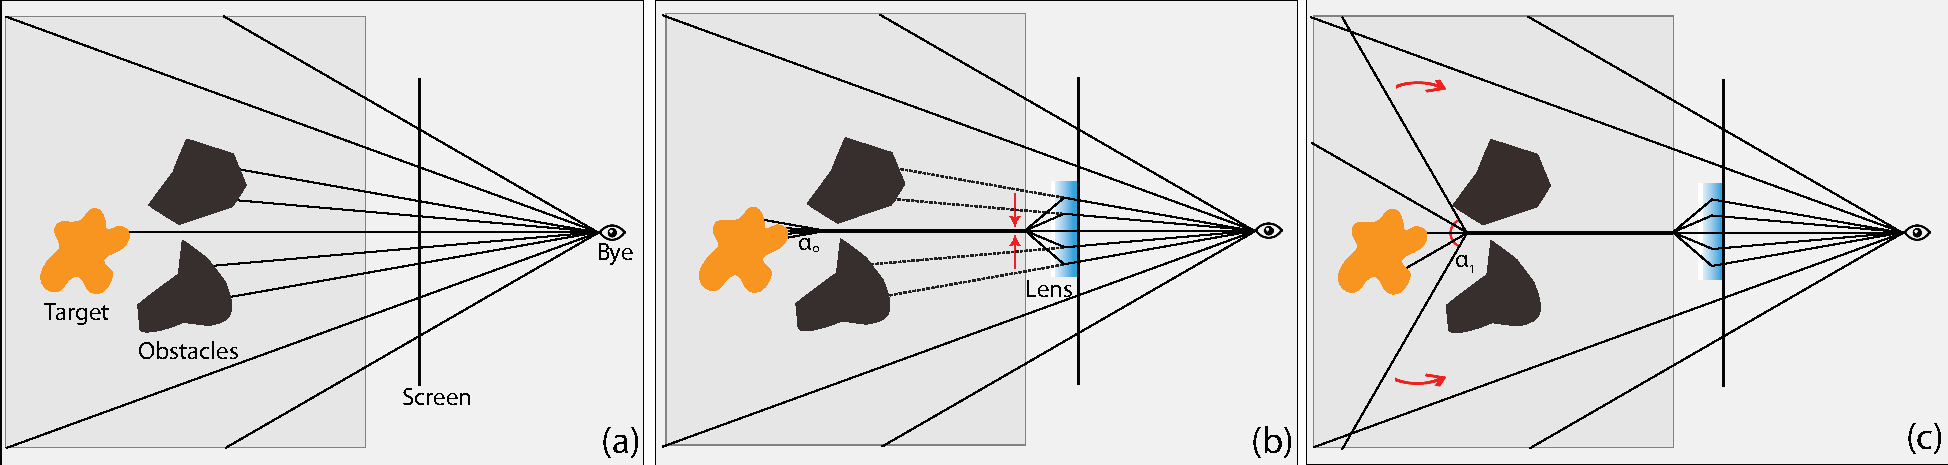
\includegraphics [width=0.8\textwidth]{images/principle.pdf}
\vspace{-0.15cm}
\caption{Principle of the obstruction-free lens. An interesting object is partially hidden by occluders in front of it. (a) Classic raycasting result. (b) Our lens gathers the rays to avoid occluders. Once close to the target, rays follow again their initial paths. However, only a small part of the target is visible. (c) Scattering the rays makes the full target visible.}
\label{f:fisheye}
\vspace{-0.15cm}
\end{figure*}

\section{Principle}
\label{sec:principle}
%
%
Our proposed lens combines the modification of several parameters of a typical DVR rendering of volume data, as follows. Consider the typical DVR algorithm: Given a scalar volume $V \subset \mathbf{R}^3 \rightarrow \mathbf{R}$, each pixel $\mathbf{x} \in I$ in the DVR image $I \subset \mathbf{R}^2$ thereof corresponds to the compositing of sampled data along a ray starting passing through $V$ and ending at $\mathbf{x}$. In classical DVR (\autoref{f:fisheye}-a), such rays are defined by the eye position $\mathbf{e}$ and a viewing-direction unit vector $\mathbf{d} = (\mathbf{x} - \mathbf{e}) / \| \mathbf{x} - \mathbf{e} \|$ pointing from $\mathbf{e}$ to $\mathbf{x}$. Consider next a focus point $\mathbf{f} \in I$ (the \emph{lens center}) and a lens radius $R > 0$. In our proposal, we modify all rays traveling through the disk $D = \{\mathbf{x} \in I | \| \mathbf{x} - \mathbf{f} \| \leq R\}$, or \emph{focus area}, in order to de-occlude, magnify, and emphasize a target object. Our new ray behavior can be divided into three steps: (1) Provide an unobstructed view of the occluded object. This moves closer to the target while avoiding the obstacles by pushing them aside. (2) Set a wide field-of-view (fisheye) to better see the target. (3) Interactively modify various parameters of the lens, lighting, and opacity TF in real time to better explore the target. These steps are detailed next.

\subsection{Creating an unobstructed view}
\label{sec:gathering}
%
The scenario our lens addresses is as follows: Given a volume $V$, users produce a DVR thereof, using whatever suitable TFs and other parameters are applicable. When examining $V$ from various viewpoints, (at least) one viewpoint $(\mathbf{e},\mathbf{d})$ is found from which some intriguing structure is \emph{partially} visible in $I$. We call this structure the \emph{target}. Users next want to quickly and easily unravel the target. For this, we proceed as follows: We first \emph{gather} all rays passing through the lens pixels (focus area $D$) to follow the lens' axis vector $\mathbf{a} = (\mathbf{f} - \mathbf{e}) / \| \mathbf{f} - \mathbf{e} \|$. As explained above, at the location $\mathbf{f}$ of the lens center, we do see an interesting partially occluded target. Hence, by definition, the gathered rays pass \emph{through} occluders to hit this target, otherwise we would not see it. We control gathering by setting the ray direction passing through $\mathbf{x} \in D$ to $\mathbf{r}(\mathbf{x}) = (1-\alpha) \mathbf{a} + \alpha \mathbf{d}$, with $\alpha \in [0,1]$. When $\alpha=0$ (default value), all rays follow the lens axis $\mathbf{a}$, thus, can best pass through obstacles. When $\alpha=1$, rays follow their original classical DVR path. Changing $\alpha$ with the mouse wheel allows one to smoothly navigate between the lens effect, \emph{i.e.} opening up a `hole' in the volume to see the target, and a classical DVR visualizaton of the volume.
%
\subsection{Setting a wide field of view}
%
Once the rays pass obstacles (Sec.~\ref{sec:gathering}), we want to \emph{scatter} them so as to best sample the target. Consider that this target is at some depth $t_{target}>0$ within $V$. After the rays pass the occluders, but before they hit the target, \emph{i.e.}, travel past a distance $t_{min} < t_{target}$ through $V$, we deflect (scatter) them so as to best sample the target. For this, we set the parametric position of a ray point to $\mathbf{p}(\mathbf{x}, t) = \mathbf{r}(\mathbf{x})t + \beta (\mathbf{x}-\mathbf{f})(t-t_{min})$ for any pixel $\mathbf{x} \in D$ and any $t \geq t_{min}$. Here, $\beta \geq 0$ controls the ray scattering: Small values magnify a small volume area located close to the ray $\mathbf{r}(\mathbf{x})$; larger values sample more of the volume area behind the lens. Intuitively, this works as if we moved a maginfying lens to a depth $t_{min}$ inside $V$. Summarizing, after the user finds an interesting but partially occluded target using \emph{standard} DVR, the lens squeezes rays to pass between occluders and next fans them out to reveal the target in full detail. The parameter $\beta$ can be adjusted by the user via the mouse scroll wheel while pressing the Shift key (\autoref{f:fisheye}-c).
%
%
\begin{figure}[htbp]
\centering
\includegraphics [width=0.4\textwidth]{images/bagage_orientation_bis.pdf}
\caption{A baggage presented under two different perspectives. (a) The baggage is composed by various type of items. the camera is located at the top front of the baggage. (b) The camera is located at the baggage side.}
\label{f:baggage_orientation}
\end{figure}

\subsection{Interactive exploration of the target}
%
We allow users to interactively modify several parameters of the DVR and the lens to achieve a more effective exploration, as follows.

\vspace{0.2cm}
\noindent\textbf{Lens radius:} The lens radius $R$ can be controlled via the mouse wheel, thereby specifying how big is the `hole' to open up in the volume to see the target. The parameters $\alpha$ and $\beta$ controlling respectively the gathering and scattering of rays are controlled by the mouse wheel and modified keys. The value $t_{min}$ controlling the depth from which scattering starts is controlled using the arrow keys.

\vspace{0.2cm}
\noindent\textbf{Lens axis:} Users can rotate the lens axis $\mathbf{a}$ using a virtual trackball activated by the right mouse button. Changing this direction effectively samples the target from all possible viewpoints, thereby allowing the user to look `around' it so as to see its parts which are not visible from the current viewpoint, but \emph{without} having to actually change the viewpoint. This is very important, since changing the viewpoint may bring us to a situation from where the target is completely invisible, so we do not know where precisely to activate the lens any more.

\vspace{0.2cm}
\noindent\textbf{Lighting:} We modify the volumetric Phong lighting parameters to better explore the target, as follows. Let $d(\mathbf{x})$ be the distance from a voxel $\mathbf{x}$ to the target center $\mathbf{e} + \mathbf{a}t_{min}$. Let $\phi$ be the specular term coefficient, set by default to a high value. First, for all voxels $\mathbf{x} \in V$ that project in the lens ($d(\mathbf{x}) \leq R$), we use a specular coefficient $\phi(\mathbf{x}) = \phi (1-d)/R$; all voxels projecting outside the lens lens ($d(\mathbf{x}) > R$) use a value $\phi(\mathbf{x}) = 0$. Hence, voxels close to the lens center appear specular, while voxels outside the lens appear diffuse. Secondly, we allow the user to rotate the light vector using the same trackball mechanism as for the lens axis rotation. These two mechanisms combined realize the effect of a moving flashlight turning around a shiny target. This highlights small-scale details on the target surface, again, without having to change the viewpoint or lens location.

\vspace{0.2cm}
\noindent\textbf{Opacity:} Finally, we modify the opacity transfer function as follows. Let $TF_{o} : \mathbf{R} \rightarrow [0,1]$ be the user-chosen opacity function. Let  $TF^{lens}_{o}$ be an opacity function computed by adding to $TF_{o}$ a Gaussian pulse centered at the average density value $\rho$ in the target. Then, for each voxel $\mathbf{x}$ projecting in the lens, we use an effective transfer function $TF(\mathbf{x}) = TF_{o} d/R + TF^{lens}_{o} (1-d)/R$; for voxels projecting outside the lens, we use $TF_{o}$. The effect is that voxels in a ball or radius $R$ around the target will become less transparent, thus more visible. However, voxels having the same densities but outside this ball will use the default transfer function (which could make them transparent). This allows to have voxels with similar densities either opaque (if they are close to the target, thus interesting) or transparent (if they are \emph{e.g.} in front of the target, thus occluding).


\subsection{Smooth transitions}
\label{continuity}
%
Our ray trajectories create discontinuities at the lens border. We propose a solution as follows. All rays traveling through the lens have trajectories and behaviors very different from those which never cross this lens. Without any additional post-treatment, the previous steps create discontinuities at the boundary of the lens. To address this issue we use an interpolation function between the final ray trajectory and the one before the previous steps. In fact, the closer a ray is to the lens border, the closer is new trajectory will be to the previous one. This interpolation offers a smoother transition between the lens viewport and the rest of the volume. This linear interpolation $p\left(k\right)$ between the new position $p^{1}$ of a sample along the ray and the one if it was not modified by the lens $p^{0}$ can described as: $p\left(k\right) = p^{0} + f\left(k\right)\left( p^{1} - p^{0} \right)$ where $k \in  \left[0,1\right]$  is the normalized distance to the axis of the lens and $ f\left(k\right)\in  \left[0,1\right]$ is a function that modifies the speed of the interpolation. For instance, we used $ f\left(k\right) = k^2$ in order to reduce the interpolation near the center of the lens.

Algorithm \ref{alg:propagation} shows a pseudo code of the behavior of our deforming lens


\begin{algorithm}
\SetKwInOut{Input}{Input}
\SetKwInOut{Output}{output}
\SetKwInOut{Parameter}{Parameter}

 \Input{
 $\vec{e}$: the eye position,
 
 $\vec{d}\left(x,y\right)$: the ray direction according to the screen space coordinates of the resulting pixel ($x$ and $y$),
 
 $step$: the sampling distance along the ray.
 
 }
 \KwResult{the pixel color.}
 
 \Parameter{
 $a$: the attraction factor,
 
 $\alpha$: the angle of view.
 }
\BlankLine
 
  $k  \leftarrow $ the normalized distance to the axis of the lens
 $\vec{p}_{near}  \leftarrow \vec{e} + t_{near} \times \vec{d}\left(x,y\right)$ //The initial position  \; 
 $\vec{p}^{0} \leftarrow \vec{p}_{near} $ \; 
 \While{ $ t \le t_{far}$ And $Opacity \le Opacity Threshold  $ }{
 	\If{the current ray is inside the lens}{
    	\If{ $t < t_{target}$ }{
        	$\vec{p}^{1} \leftarrow \vec{p}_{near}\left(x,y\right) + t \times \vec{d}_{target} + a \times \vec{f}_{attraction}$  \;
            \lElse{
        	$\vec{p}^{1} \leftarrow \vec{p}_{target} + \left( t-t_{target} \right) \times \vec{d}_{fishEye}\left( \alpha \right)$
        	}	
        }
               
    $\vec{p} \leftarrow \vec{p}^{0} + f\left(k\right) \times \left( \vec{p}^{1} - \vec{p}^{0} \right) $	\;
     \lElse{
     	 $\vec{p} \leftarrow \vec{p}^{0}$
     }
    }
\emph{Sampling at the position $\vec{p} $ }\;
    
    \emph{Shading the sampled value }\;
    
    \emph{ Compositing the shaded sampling point with the previous values} \;
 
    $t \leftarrow t + step$ \;
    $p^{0} \leftarrow p^{0} + step \times \vec{d}\left(x,y\right)$ \;

}
$color_{final} \leftarrow$ composited colors \;
return $color$
 

\label{alg:propagation}
 \caption{Pseudo code of our lens deformation algorithm}
\end{algorithm}


\begin{figure*} 
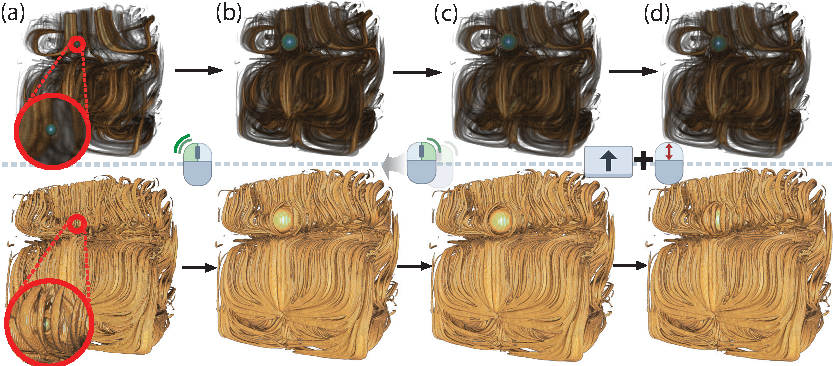
\includegraphics [width=\textwidth]{images/stream_lens.pdf} 
\caption{ A spherical item and its surrounding area are inspected using to our lens with 2 different transfer functions. The first part is displayed with transparency in opposition to the part below. The opacity helps to see the shape of the surrounding whirlpool. (a-a') The streamline dataset displayed using our framework. A dense object is hidden inside a whirlpool. (b-b') The lens tool is applied to the partially hidden object (double-click). The area is magnified and the occluding part of the whirlpool located in front of the spherical item is pushed aside. (c-c') The directions of the rays inside the lens are modified to see the whole sphere through the lens (right click+ mouse drag toward the desired direction). (d-d') The occluding part of the whirlpool can be restored/pushed gradually while keeping the area magnified (Shift + scroll).  }
\label{f:stream_lens}
\end{figure*}

\begin{figure} 
\includegraphics [width=0.45\textwidth]{images/streamline_orientation.pdf} 
\caption{ This figure shows 2 visualizations of a streamlines dataset. (a) The transfer function used allows to spot a spherical dense item inside the volume thanks to transparency. (b) This spherical object become occluded when the opacity of the surrounding whirlpool is increased in order to analyze its shape and behavior. }
\label{f:streamLineSTDViz}
\end{figure}
After the selection of a target, the lens offers a smooth transition between the previous view and the new one using a  slow-in/slow-out technique~\cite{Dragicevic:2011:TDA:1978942.1979233}. With this animation, the increase of the gradual speed at the beginning of the animation helps the user to start tracking the moving obstacles, and the decreasing speed at the end allows the user to predict where these occluding items stop moving. This also gives some semantic to the moving shapes, allowing the human mind to interpret the motion as a magnification of a target, and to keep the focus on visual entities during this transition. 



Moving objects are entities that change locations in space over time. This is the case with aircraft trajectories where an aircraft takes off at a given airport at the beginning of its strip and lands onto another one at the end of its journey. Classical methods use projected lines on a 2D visualization to explore dataset composed of such moving objects \cite{hurter2014interactive}. Even if such methods have shown valuable results, additional insight and data retrieval can be envisaged with other rendering techniques like volume rendering.

\textbf{Dataset rasterization:} While Bresenham's line algorithm is a standard algorithm to turn a line form the vector space to a raster 2D or 3D space, it will not fulfill volume rendering compatibility. Raster line must have a given thickness to maximize the number of intercepting rays and thus ensuring their visualization thanks to volume rendering methods. Other techniques can be envisaged with the computation of meshes (i.e. pipes that encompasses the 3D line) but such computation can create geometric artifacts and might be long to process. Therefore, we used an extended version of the kernel density estimation algorithm \cite{ silverman1986density} into a 3D space. Such method has already shown interesting results with visual simplification and trajectory aggregation \cite{hurter2012graph} and is part of so-called pixel-based visualization \cite{hurter2015image}.
Such process works as follows: we first define a 3D Gaussian kernel of a radius R; the center of this kernel has the highest value, while its border the lowest. Second, we re-sample every trajectory with a minimum distance between two consecutive points inferior to the half of the kernel radius. Third, we compute the convolution of this 3D kernel with the re-sampled trajectories.

Convolution can take time with a large dataset to process, therefore, we turned this computation into the frequential space. Such technique has already been applied with trajectory dataset and can even be accelerated thanks to GPU techniques \cite{lhuillier2017ffteb}.

\section{Application Scenarios}
\label{sec:scenarios}
%
We next demonstrate our obstruction-free lens via five use-cases considering scalar density volumes from baggage inspection, 3D flow simulation, radiology, air traffic planning, and diffusion tensor imaging.

\subsection{Baggage inspection: An unusual blunt object}
\label{sec:baggage}
%
In most airports, security agents deal with volumetric data exploration during baggage inspections. While automatic systems are now able to detect densities of harmful substances such as C-4, TNT, and nitroglycerin, and even some prohibited articles such as classical firearms and knives, it remains difficult to identify unusual threats. In addition, baggage inspection faces four main concealment strategies\,\cite{7819413}:

\vspace{0.15cm}
\noindent\textbf{Superposition}: A threat (prohibited object) may be sheltered among dense materials. It is sometimes possible to see through such a `shield' using high penetration (enhanced X-ray power) or image processing (contrast improvement) techniques. However, such techniques are not universally available and also require fine-tuning various parameters, which slows down the inspection process.

\vspace{0.15cm}
\noindent\textbf{Location}: Depending on its location inside the luggage, a threat can be hard to detect. Objects located in the corners, edges, or in the luggage'��s frame are very hard to spot.

\vspace{0.15cm}
\noindent\textbf{Dissociation}: One can conceal a threat by spreading its parts in the luggage, \emph{e.g}, by disassembling a weapon and scattering its parts.

\vspace{0.15cm}
\noindent\textbf{Lure}: A lure can be used to to hide the real threat. For instance, a minor threat like a small scissors can be clearly visible and catch the security agent's attention while a more important threat remains hidden.

Baggage labeled as suspicious either by human inspection or automated scan heuristics need detailed human investigation. Besides physical unpacking, which is time-consuming, one can use `virtual unpacking' tools that segment the 3D scan by a density-based confidence measure and next move the segmented objects away by animation to reduce occlusion\,\cite{Li:2012:LVV:2425296.2425325}. Such systems have been patented and used in production\,\cite{patent}. An important limitation thereof is that, when the automatic segmentation is not optimal, the user needs to manually change its parameters, repeat it, and repeat the animation, which goes back to being time consuming.

Consider the baggage scan in \autoref{f:baggage_lens} with a volume size of 283x189x344 voxels. Automatic baggage inspection systems will not detect anything suspect on this scan. However, while visually exploring this baggage from different angles (\autoref{f:baggage_lens}a-c), it appears that an object is hidden between a set of mugs. A common solution to this type of issue in baggage inspection is to filter materials by density in order to show or hide subsets of the volume and reduce the occlusion. However, in this case, this solution does not work, as the suspect target has almost the same density as the surrounding mugs. Hence, removing the occluders will also remove the target (\autoref{f:baggage_lens}d-f). Using the obstruction-free fish-eye lens helps in this kind of situation. Clicking on the sharp detail visible in \autoref{f:baggage_lens}c first gathers rays so they pass through the low-density zone between the mugs (\autoref{f:baggage_lens}f)

The user has just to use this tool on the partially hidden target. Then, a transition inside the lens will start and smoothly provide the final unobstructed view of the blunt object which is, in this case, a ceramic shuriken (\autoref{f:baggage_lens}e-g). However, this shows only a small part of the target. Scattering rays next fully reveals the target (\autoref{f:baggage_lens}h). The user can adjust the lens size to get a more detailed view of the target (\autoref{f:baggage_lens}i). Next, the user can locally turn the viewpoint around the target, as already shown in \autoref{f:rotation}. From these views, the controller decides that the target is a copy of a shuriken (Japanese ninja star weapon). However, since the object is very thick and blunt (see \autoref{f:rotation}), it is clearly not a threat.

As we obtained this dataset from an airport, we had the opportunity to get feedback on our obstruction-free lens from three baggage security operators. According to them, our tool is interesting as it can provide them a better perception of the items inside the baggage as compared to the classical 2D single-viewpoint X-ray machinery they commonly use. However, this tool should not be used for the typical carry-on baggage inspection where the time-window allowed for inspection is extremely small (about 15 to 20 seconds) in order to keep a smooth traffic flow, for economic reasons. In contrast, this tool is considerably more interesting for inspecting checked-in baggage, where one has a longer inspection time-window (up to 3 minutes). The added value for this use-case is also higher: Opening up checked-in baggage for manual inspection is much more complicated and time-consuming than for carry-on baggage, given its automatic handling. Moreover, the only system for inspecting such baggage currently in use is a scanner that aims to automatically detect suspicious objects in X-ray imagery; this system suffers from false positives, so having a manual in-depth examination tool like our lens can quickly eliminate such false positives, and thus the unnecessary delays they cause when opening up the respective baggage.

\subsection{Fluid flow: A deep-buried spherical vortex}
\label{sec:flow}
%
%
Flow visualization using streamlines has a long history in scientific visualization~\cite{brambilla2012illustrative,merzkirch2012flow}. When applied to 3D datasets, a key challenge is to balance the streamline density. Low values allow seeing inner regions in the data but can subsample (miss) important patterns. High values show more data but create too much occlusion. We next show how our lens can be used to discover interesting patterns in the second case, \emph{i.e.}, a 3D volume densely filled with streamlines. The dataset, introduced in\,\cite{griebel2004flow}, captures the simulation of water flow in a basin computed on a grid of 128x85x42 cells. A set of 4595 streamlines with 183K sample points is next traced by pseudo-random seeding over this vector field. We convert this set of 3D curves (polylines) to a scalar volume by using kernel density estimation (KDE)\,\cite{silverman1986density}. Similar techniques have been used to compute density maps of 2D trail-sets\,\cite{hurter2012graph,cubu,hurter2015image}. To increase computational speed, we compute the KDE in the frequency space and using GPU acceleration, following\,\cite{lhuillier2017ffteb}. The resulting volumes have a resolution of $500^3$ voxels and can be directly displayed using DVR (\autoref{f:stream_lens}). Note that, given the smoothing effect of KDE, streamlines appear now as finite-thickness tubes rather than pixel-thin curves.

For a first overview, we display the volume using standard DVR. After turning the viewpoint a bit, we notice a dense spherical item inside the dataset (\autoref{f:stream_lens}a). To see its shape better, we increase the opacity; however, this immediately increases occlusion so the item becomes invisible. Conversely, decreasing opacity to reduce occlusion makes the item almost transparent. Our lens solves the problem: In the initial view (\autoref{f:stream_lens}a), we point at the target and turn on the lens. This effectively pushes away the occluding stream bundles, and lets us see that our item is nearly perfectly spherical (\autoref{f:stream_lens}b). This is something we could not have assessed from \emph{any} viewpoint and with likely any opacity modulation using standard DVR. Our object is a set of densely-packed, low-speed, tightly-turning streamlines that create a ball-like vortex. Interestingly, this spherical vortex has not been discovered by any of the visualization techniques that we are aware of that used this same dataset\,\cite{telea_vis_99,griebel2004flow,ddh,lhuillier2017ffteb}. To make sure our target is spherical, we view it in the lens from different directions, by interactively changing the ray directions in the lens (\autoref{f:stream_lens}c). Finally, we can close the lens but keep the target magnified (\autoref{f:stream_lens}d).


\begin{figure*}[htb]
\centering
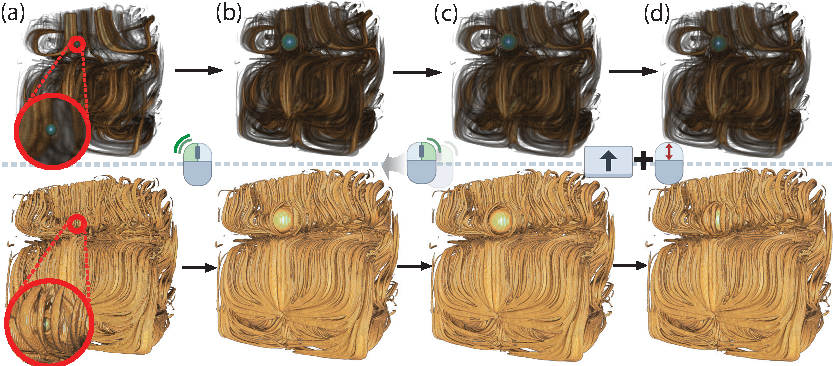
\includegraphics [width=0.95\textwidth]{images/stream_lens.eps}
\vspace{-0.15cm}
\caption{Flow volume exploration with two different opacity transfer functions (top and bottom rows). In viewpoint (a), we notice a small high-density spherical item. (b) We apply the lens at that location (double click). (c) The directions of rays in the lens are changed to see the whole target in the lens (right click + mouse drag change direction). (d) The lens is gradually closed while keeping the focus area magnified (shift + scroll).}
\vspace{-0.15cm}
\label{f:stream_lens}
\end{figure*}

\subsection{Chest scan: A hard to see tumor}
\label{sec:chest}
%
In our third use-case, we consider a contrast chest CT scan (512x512x110 voxels) of an elderly patient having a sizeable lung tumor. The tumor was detected at a CT scan ordered by the pulmonologist in charge of the patient, after the patient reported acute chest pain. Typical examination of these scans by the pulmonologist and radiologist in charge involves slice-based views. Figures~\ref{f:slicer}a-c and \ref{f:slicer}d-f show two such slice sets (axial, coronal, and saggital views), produced using typical lung, respectively mediastinal, contrast presets. Although the tumor is visible in all these views, its exact shape, morphology, and connection to the lung walls are not easy to assess. Finding such details on the tumor is essential, explained both doctors in charge, for determining the TNM score and also planning treatment. Using standard DVR makes the tumor and its 3D position partially visible (\autoref{f:slicer}f). However, occlusion from the rib cage and other tissues is still present. Using both TF presets and manually changing the TFs in the 3D Slicer tool\,\cite{slicer} used to create the DVR could not help de-occluding the tumor without making (parts of) it transparent. This is also visible in the slice images in \autoref{f:slicer}a-f, where the gray values for the tumor and surrounding skin-and-muscle tissue on the rib cage are very similar. 
This density similarity is due to the fact that the tumor had grown rapidly in a short time span, explained the pulmonologist. As such, the tumor started necrotizing, which filled it with fluids, making its density very similar to that of the obstructing (skin and muscle) tissue. In conclusion, one cannot remove such occluding tissue in a classical DVR setting by opacity TF manipulation without also removing the tumor. This situation makes examining this specific tumor harder than for regular cases.

\begin{figure}[htb]
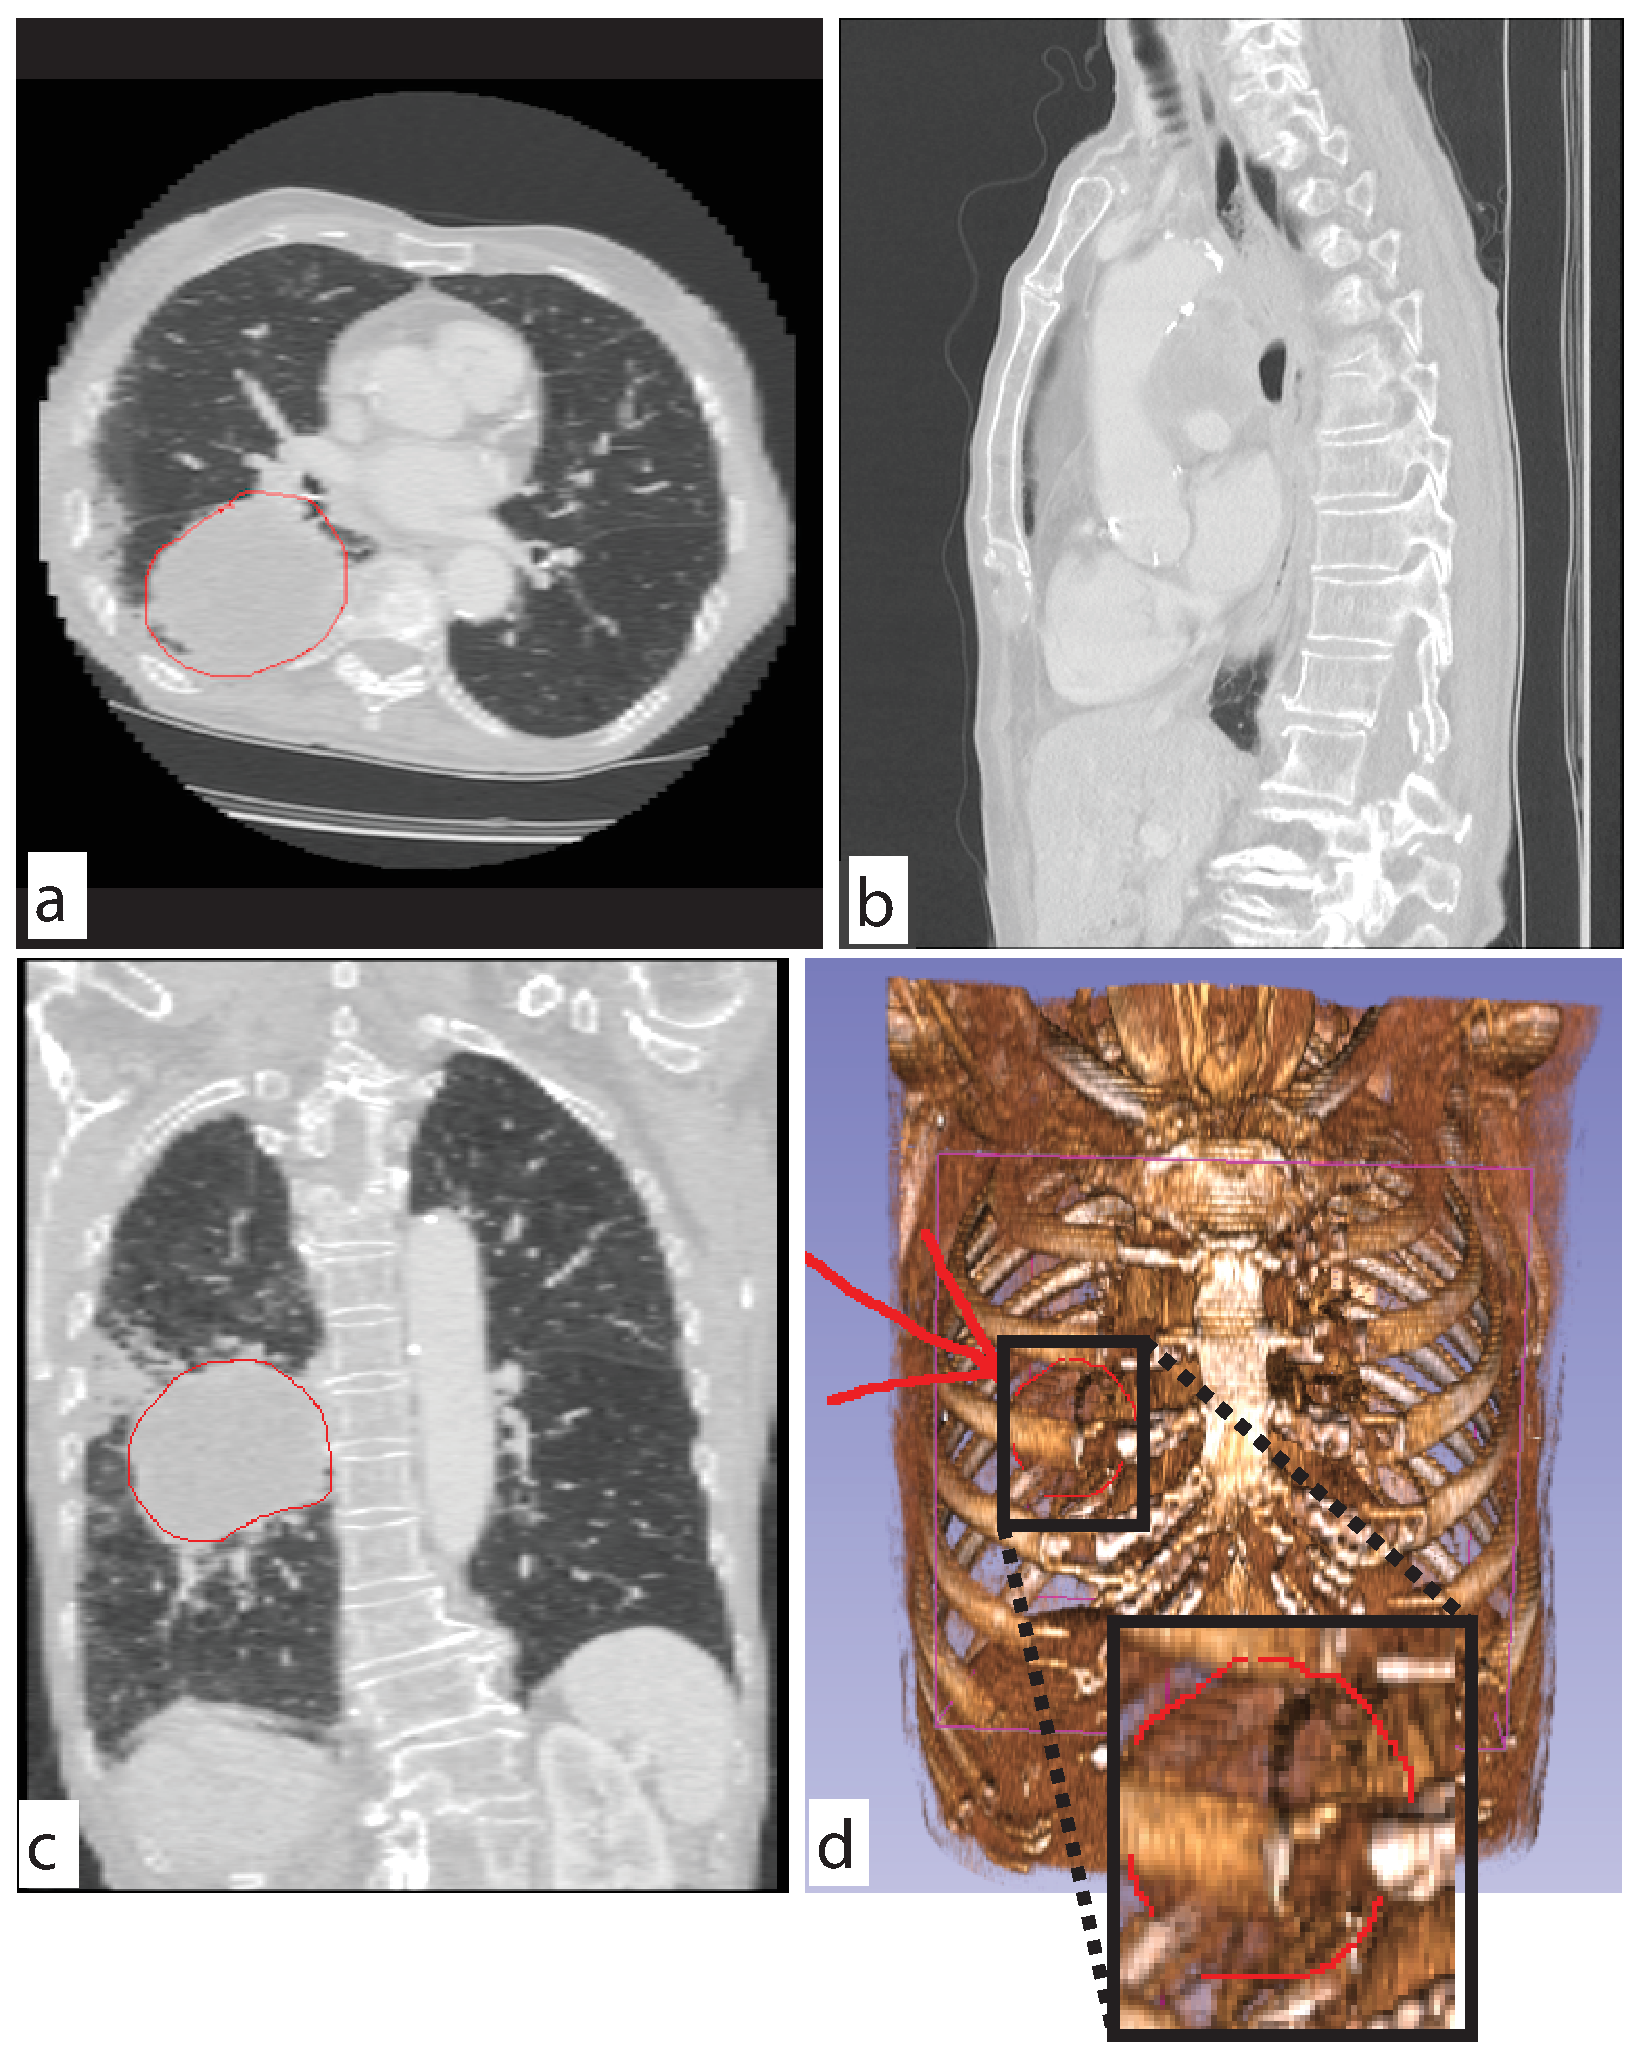
\includegraphics [width=0.48\textwidth]{images/slicer.eps}
\caption{Lung tumor visualization using slices (a-c) and standard DVR (d). Annotations are manually added by the examiner to delineate the tumor location. Images constructed using the 3D Slicer tool\,\cite{slicer}.}
\label{f:slicer}
\end{figure}

We next used our lens to examine the tumor. Sample snapshots obtained in this process are shown in \autoref{f:params}. Comparing these with standard DVR (\autoref{f:slicer}d), several points can be made. First, the tumor is significantly more visible when using the lens, both in terms of removing the occluding tissue and in terms of the tumor's opacity -- compare the inset in \autoref{f:slicer}d with the images in \autoref{f:params}. Secondly, relighting the tumor from various directions allows one to see small-scale morphological details such as the tumor's surface shape and its connection via protuberances and veins with the lung walls.

To assess the added-value of our lens, we asked the two medical specialists (pulmonologist and radiologist) involved in treating the patient that this dataset came from to study the lens' features and state its potential advantages and/or limitations as compared to standard slicing and DVR techniques they use in their practice. Both specialists have over 10 years of medical experience in treating lung cancer, and routinely use several slicing and DVR software tools. They work in a private hospital in Belgium and are not actively associated to medical imaging research. Moreover, our (authors') identities were hidden from them, by using a third person in the communication. The provided input can be summarized as follows: The occlusion-free lens is definitely easier and faster to use than classical DVR and/or slicing techniques. It is especially more effective than these to get a quick, first impression of a deep buried anatomical detail. Changing the lens' parameters by direct interaction is as simple as changing window/level functions in a typical slice-based visualization, and is definitely simpler than tuning typical DVR parameters to obtain similar results. This `entices' the user to explore, which is a good aspect. The fact that the lens minimizes viewpoint change (volume rotation), \emph{i.e.}, after a suitable viewpoint was found from which a (small) part of the target is visible, one doesn't need to change this viewpoint, is a strong feature, as 3D viewpoint changes are disruptive and cost time. This is important in a cost-aware environment where specialists have very limited time (10-15 minutes) to  assess a CT scan. However, the lens cannot and should not replace classical slice-based investigation, which shows small-scale details better. This is especially important when examining small-size lesions, tumors, or other similar anatomical features, that the lens will arguably not be able to help with, as these are too small in the first place to attract the attention of the examiner looking at a standard DVR rendering. In the context of the current dataset (Fig.~\ref{f:slicer}), the lens was useful to both confirm the TNM score (T3 grade tumor, 6.5 cm in size) found via the 2D slices, but much more so for inderstanding how and where the tumor is connected to surrounding tissue, which is very hard to do using only 2D slices.

\begin{figure}
\centering
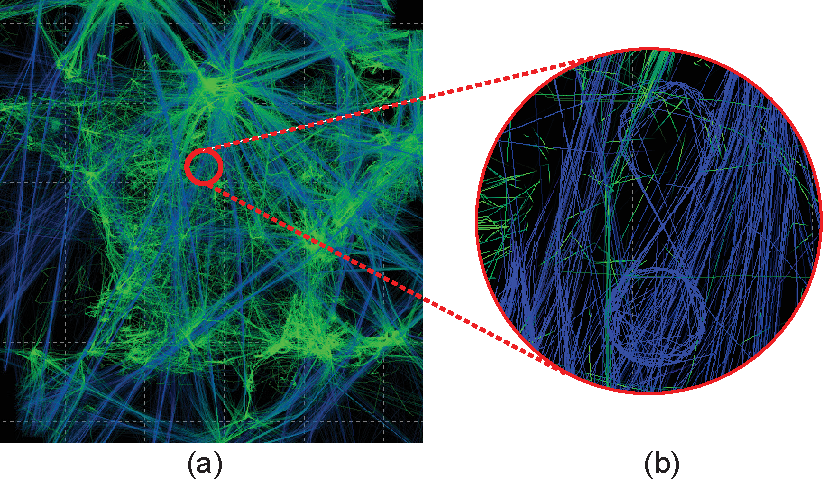
\includegraphics [width=0.48\textwidth]{images/aircraft.pdf}
\vspace{-0.15cm}
\caption{Visualizing one day of aircraft trajectories over France\,\cite{hurter2009fromdady}. (a) Overview of all trails. (b) Zoom, filtering, and color mapping techniques are used to highlight an outlier trajectory of an aircraft performing an eight-shaped loop. Revealing this outlier costs significant user effort.}
\label{f:fromdady}
\vspace{-0.15cm}
\end{figure}


\subsection{Aircraft trajectories: Outliers in the French sky}
\label{sec:atc}
%
%
We next consider a task from the air traffic planning field -- detecting and studying outliers in large-scale datasets containing tens of thousands of 3D (latitude, longitude, height) trails of aircraft over a given spatio-temporal region\,\cite{hurter2014interactive}. Typically, such datasets are displayed using 2D (latitude, longitude) plots where opacity encodes the spatial density of flights. \autoref{f:fromdady}-a shows one day of recorded aircraft trajectories over the French air space using this 2D technique. \autoref{f:fromdady}(b) shows a detail zoom-in of this dataset, where we can see an abnormal -- that is, far from straight or slightly curved -- aircraft trajectory: A tanker aircraft performed an eight-shaped loop as it was waiting to refuel other aircraft. Revealing such patterns using 2D techniques, \emph{e.g.} \cite{hurter2009fromdady}, is very hard. In particular, it is hard to de-occlude these patterns from the overall context of criss-crossing aircraft trails, even when one knows their 2D spatial location.

Our lens can help for this task, as follows. We first convert the set of 3D trails to a $500^3$ density volume, using KDE as described for the streamline use-case (Sec.~\ref{sec:flow}). Examining this volume using standard DVR allows us to see that there is an outliner (that is, not straight) trail at some point in space, see curved patterns in \autoref{f:aircraft_lens}a. By activating the lens on this area and interactively tuning the target depth $t_{min}$ (since we don't know the height of this trail), we can quickly obtain a view where the outlier trajectory is in focus and the occluding ones are pushed away (\autoref{f:aircraft_lens}a). Finally, just as in the other examples presented so far, the user can quickly change the magnification factor and view direction to better study this trajectory in context (\autoref{f:aircraft_lens}b-d). From these images, one directly and easily sees that the outlier trajectory has an eight shape. Revealing this outlier trail using standard 2D visualization techniques\,\cite{hurter2009fromdady} costs several minutes. Doing the same using our lens approach costs under one minute, for the same users. Additionally, if we compare Figs.~\ref{f:fromdady}b and~\ref{f:aircraft_lens}b-d, we argue that the eight-shape of the outlier trajectory is much more prominent, and thus recognizable, in the latter images (using our lens) than in the former ones. Last but definitely not least: The 3D volume rendering approach that our lens is based on explicitly encodes the flight height information, so our lens can use it by interactively tuning the depth value $t_{min}$ where the lens is focused. This is not possible with 2D techniques which ignore this depth dimension.

We validated our findings with an air traffic data scientist with more than 10 year experience in air traffic control and air traffic planing. She confirmed that this specific eight-shape trail in \autoref{f:fromdady}(b) is an actual aircraft which performed waiting loops and acted as a fuel supplier for military aircraft. Other comments included the following: Compared to standard 2D visualization techniques, our tool makes detecting outliers easy since there is no need for complex manipulation to reveal such outlier trails. Also, the user does not have to deal with color and alpha mapping parameter-tuning to make specific outliers emerge. Separately, trail visualization easily creates many occlusions leading to either fully opaque areas or too much local overlap, both which hinder seeing and examining specific trails. Our lens does help such cases by distorting the space to locally remove such occlusions. All in all, in the studied dataset (\autoref{f:fromdady}), the lens was specifically useful since, for high transparency, one would not detect the outlier trail, while for low transparency, one would get a hint of the outlier's existence, but not see it in detail due to too much occlusion; the lens allows using low transparency, but removes the clutter caused by it to reveal the outlier.


\begin{figure*}[htbp]
\includegraphics [width=0.98\textwidth]{images/aircraft_lens.pdf}
\caption{Inspecting an abnormal aircraft trail. (a) The abnormal trail is spotted in an all-trails view as it is highly curved while all other trails are relatively straight. Activating the lens at the outlier location (b) and changing the magnification factor (c) reveals the trail's eight-shape. (d) Rotating the viewpoint provides spatial insight on the embedding of the outlier in the surrounding trails.}
\label{f:aircraft_lens}
\end{figure*}
%

\subsection{Brain fibers: Uncluttering the bridge}
\label{sec:dti}
%
Finally, we consider a last example related to the exploration of fiber tracts visualized as streamlines of the major eigenvector of a diffusion tensor imaging (DTI) field. Such datasets shows a spatially complex structure which makes them hard to explore\,\cite{assaf08}. In particular, fiber tracts are spread volumetrically over the entire extent of the brain, and create tangled patterns which make it very hard to see deep within the emerging structures. DVR techniques are often used to render such fiber tracts, one of the advantages being that close fibers get visually `merged' to reveal spatially coherent structures, an effect which is not possible when fibers are rendered using polyline (streamline-like) representations. However, DVR methods also create more occlusion, thus difficulties in seeing structures deep within the volume.

For this use-case, we use an $128\times128\times51$ DTI volume ( same dataset as in~\cite{everts15}). From this volume, we traced 150352 fibers seeded in, and going over, regions of high fractional anisotropy. Next, we filtered out fibers shorter than 2mm, yielding a total of 120593 fibers to display (6.4M sample points). Next, we converted this fiber-set to a $512^3$ density volume, using kernel density estimation with a 3D isotropic kernel of radius 15 pixels. The conversion process is identical to the one used for the streamlines in Sec.~\ref{sec:flow}. Figure~\ref{fig:dti}a shows the result, rendered with DVR, with a simple opacity function mapping the fiber density. While terminal fibers are well visible, it is impossible to discern anything inside the volume. Activating the lens in the middle of the volume opens a hole through which a small part of the \emph{corpus callosum}, the fiber bundle wrapping the bridge that connects the two emispheres, becomes visible. To obtain an even better view hereof, we slightly decrease the opacity (Fig.~\ref{fig:dti}c). The \emph{corpus callosum} is now clearly visible, appearing as a compact structure, due to the KDE blending of neighbor fibers. Note that obtaining such a view on the \emph{corpus callosum} using only DVR would be very hard, since transfer functions would either render separated (non-merged) fibers, or else make the fibers surrounding the structure of interest too thick and occluding. 

There is one notable difference to this scenario as compared to all previous ones. In all earlier cases, the standard DVR of the data (that is, without the activated lens) showed us a partial small cue of the structure of interest within the volume, and we used the screen-space location of this structure as the center point where to activate the lens. In this last scenario, there is no clear point within the original DVR image (Fig.~\ref{fig:dti}a) from which the \emph{corpus callosum} is even partially visible, due to the high opacity given by the transfer function used. As such, the user activates the lens here at \emph{any} desired point to peek inside, and towards the center of, the volume. However, given the nature of the data, the structure of interest is quite easily visible from most such viewpoints (see lens inset in Fig.~\ref{fig:dti}b). Once its presence is revealed, the user can next adjust the viewpoint and/or the opacity transfer function to get an optimal view on the target, such as the one shown in Fig.~\ref{fig:dti}c.

\begin{figure}[htbp!]
\centering
\includegraphics [width=0.45\textwidth]{images/dti.eps}
\caption{Revealing the \emph{corpus callosum} in a DVR of a set of DTI tracts.}
\label{fig:dti}
\end{figure}


%

\section{Discussion}
In this paper, we presented four different scenarios where we showed how our lens is a fast and flexible way to overcome occlusion issues: the exploration of a heterogeneous data-set (baggage inspection), the analysis of a deep-buried spherical vortex (fluid flow), the visualization of a hard-to-see lung tumor , and the exploration of a special aircraft trajectory.    

Nevertheless, some aspects of the lens we presented throughout this document suffers from some limitations which we detail in the following. 


First, keeping the continuity between the inner part of the lens and the rest of the volume is very important to preserve a good understanding of object deformations. This is related to the third requirement(R3) which is to keep the global context. To ensure this continuity, we used a linear interpolation function between the final ray trajectory and the one before the previous steps. In fact, the closer a ray is to the lens border, the closer is new trajectory will be to the previous one. We used linear interpolation, whose parameter was modified with a function $ f\left(k\right) = k^2$ in the purpose of reducing the interpolation near the center of the lens. Different functions and mathematical tools could have been used but the result obtained with the current function was satisfying. 

Second, we used a circular lens throughout this study. The circular shape seemed more natural for us but, we could have proposed different lens shapes. At this stage, only the radius can be increased or reduced in order to customize this shape. Furthermore, during the deformation of the rays, the shape of the items considered as obstacles and pushed aside, are modified. It would be interesting to keep their original shapes to improve this focus + context lens (R3). A solution is to adapt our rays' trajectories modification to physical based deformation inside the lens. However keeping the original shapes of all the objects that have been pushed aside can change the global context. In fact, they will either create more occlusion outside the lens or change the items' locations outside the lens by moving them away.  


Third, the angle of view in the second step of our algorithm which allows having a good sight of the targeted item and its local context can be improved. In fact, using a segmentation algorithm that computes the bounding box of the target will help to define precisely and automatically the most suitable angle of view. This is related to the first requirement(R1) which consists in giving a fast unobstructed view on the target. However, we do think it is still important to offer the possibility to modify this angle at will. In fact, this flexibility (R2) allows further exploration of the local context.

Finally, during the first main step of our lens algorithm, we try to get closer to the targeted item or area while pushing the encountered obstacles aside. Automatically finding the right distance to the target, that offers the optimum balance between a good perspective on the full target and obstacle avoidance can be sometimes difficult according to the structure of the data-set (R1 and R4). In our future works, we will instigate automatic curved rays in deforming lens in the purposes of providing in most cases a very good perspective on the target while avoiding occlusion. 

\section{Conclusions}
\label{sec:conclusions}
%
In this paper, we presented a new fish-eye-like context-and-focus lens that addresses the occlusion problems inherent in scalar volume rendering. The principle of our lens consists in first gathering (squeezing) rays so that they easily pass through occluding densities (given a user-specified opacity transfer function) and next scattering (fanning out) rays to best sample the target of interest. Our lens can be directly applied to any DVR raycaster and scalar volume dataset. Its main constraint is that the user should be able to find a viewpoint from which the target of interest, deep buried in the data, is at least slightly visible. We also present several modifications of the local rendering parameters within the lens (view direction, lighting parameters, opacity transfer function) that aim to both better separate the focus (lens) from the context (volume) and also allow more detailed examining of the target. Our lens is easy to use -- all its parameters are controlled via direct mouse-and-keyboard interaction -- and can be efficiently implemented atop of a standard GPU ray caster. Our lens is especially useful for highlighting structures of interest which are both deeply embedded in volumetric data and cannot be revealed by standard transfer function manipulations due to similar densities in the occluders and target. We demonstrate these points using five use-cases involving datasets from baggage detection, fluid visualization, air traffic control, and chest radiology, and DTI fiber tracts.

Several improvements to our proposal are possible, as follows. First and foremost, heuristics can be sought to link all our free parameters (lens size, focus depth, interpolation between focus and context) directly to the volume data, so the user interaction is minimized and therefore exploration efficiency is increased. Secondly, our lens could be extended to different types of volumetric datasets, such as multivariate (vector, tensor) fields. Last but not least, a formal wider-scale evaluation of how the lens addresses more specific tasks, and how it compares to existing tools for these tasks, such as other lens types, is a goal we aim to pursue next.

\section*{Acknowledgments}

The authors acknowledge the support of the French National Agency for Research (Agence Nationale de la Recherche ANR) under the grant ANR-14-CE24-0006-01 project ”TERANOVA” and the SESAR Research and Innovation Action Horizon 2020 under project ”MOTO” (The embodied reMOte TOwer). We also thank the pulmonology and radiology departments at the Heilig Hart Ziekenhuis, Mol, Belgium for their help with the chest tumor use-case described in Sec.~\ref{sec:chest}.




%\bibliographystyle{abbrv}
\bibliographystyle{abbrv-doi}
%\bibliographystyle{abbrv-doi-narrow}
%\bibliographystyle{abbrv-doi-hyperref}
%\bibliographystyle{abbrv-doi-hyperref-narrow}

\bibliography{template}
\end{document}

